\section{Interworking models for IoT standards}  
\label{sec:smartcity_interworking}
Interoperability means systems or products can work with other systems or products without restriction and special effort and it is the most fundamental value and a cornerstone of the open Internet~\cite{rose2015internet}. Lack of interoperability makes technical and business challenges such as increasing costs, slowing the introduction of new technologies and impossibility to connect with each other. In addition, technology cluster and data silos which cannot be communicated with other domains have been created. Therefore, it is important to make the existing IoT-based services interwork with other IoT services without changing existing systems. Furthermore, the new IoT platforms to be developed should also take interoperability issues into consideration. %However, not many IoT-enabled services are supporting interoperability among them~\cite{petrolo2014towards}.

In this regard, this section first explains interworking issues by using the two smart cities as an example. Based on that scenario, three interworking models with the aim of providing guidelines for interworking is introduced. For comparing the pros and cons of each model, an interworking model evaluation is also included.

\subsection{Towards the IoT standards interoperability}
As so far, this dissertation talks about interoperability issues but, there is no specific definition of what smart cities interoperability is. Therefore, the smart city interoperability definition is described. In addition, for more practical description, a smart city interworking scenario that is telling that why interworking between different smart cities is important is illustrated.

At present, most recent IoT-based smart cities are designed to support interoperability between IoT devices and services within the city. Therefore, data generated by an IoT device can be accessed by multiple IoT services using the same standards in the city. This is an intra-city interoperability, which is applicable within a smart city (see Fig.~\ref{fig:definition_of_smartcity_interop} (a)). However, as more people are moving between cities, and cities are connected each other, inter-city interoperability, which is supporting interoperability between connected smart cities, is becoming an important issue to be solved by IoT technologies.

\begin{figure}[H] % Add figure one
\centering
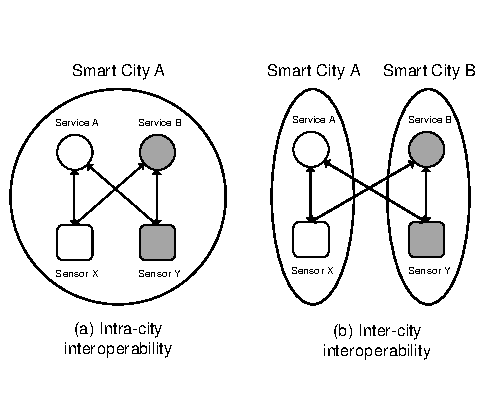
\includegraphics[width=\textwidth]{figures/fig_interoperabilities_of_smart_cities.pdf}
\caption{Interoperability of smart cities}
\label{fig:definition_of_smartcity_interop}
\end{figure}

As far as we know, most smart cities are not supporting this inter-city interoperability (see Fig.~\ref{fig:definition_of_smartcity_interop} (b)). For example, let’s consider that a smart city and its IoT platform are deployed based on NGSI like Santander. If a natural disaster is just happened in that city, a disaster management service will manage various sensors and actuators to control the traffic and alarm the citizens to be in safe places using its standards-based IoT platform (Intra-city interoperability). However, the city cannot alarm the traffic coming from other cities in which used IoT standards for platforms and devices is based on oneM2M (Inter-city interoperability). In this scenario, both smart cities need to communicate with each other to exchange information and make decisions in real time to save citizens from facing the natural disaster. Depending on the technologies used for smart city IoT service platforms and data models, inter-city interoperability can be achieved differently. If two smart cities to be connected are using proprietary IoT technologies, it is very difficult to interconnect them as their data models and APIs are all different. Either all the data stored in a city IoT platform
have to be translated into another IoT platform or all the deployed IoT services have to implement APIs for both IoT
platforms, which require huge efforts. Even in both cases, the solutions are not scalable. On the other hand, if two smart cities are developed based on the same IoT technologies, although there needs some additioanl work to be defined, inter-city interoperability can be achieved easily. In other words, for realizing inter-city interoperability between smart cities in different conditions and environment, appropriate interworking approaches have to be considered.

In the following subsection, we introduce three interworking models for achieving intra-city interoperability and inter-city interoperability. By using these models, authorities or service providers are able to interconnect their smart cities to other cities so that the coverage of smart cities can be expanded.

\subsubsection{Interworking scenario of smart cities}  
The majority of smart cities based on IoT are tailored to make the smart cities interoperable between IoT devices and services in the cities. However, since more people are traveling between cities, supporting the interoperability among cities are becoming more important and recognized as a paramount factor. In the present, there are not many IoT based smart cities that are supporting smart city interoperability~\cite{Petrolo2017}. 

Depending on the technologies used for smart city IoT service platforms and data models, Inter-city interoperability can be achieved in many ways. If two smart cities to be connected are using proprietary IoT technologies, it is very difficult to interconnect them as their data models and Application Programming Interfaces (APIs) are all different. Either all the data stored in a city IoT platform have to be translated into another IoT platform, or all the deployed IoT services have to implement APIs for both IoT platforms, which require huge efforts. On the other hand, if two smart cities are developed based on the same IoT technologies, although there needs some additional work to be defined, Inter-city interoperability can be achieved easily. In other words, for realizing Inter-city interoperability between smart cities in different conditions and environments, appropriate interworking approaches have to be considered, so three interworking models (IWMs) to solve the above issues were proposed in Fig.~\ref{fig:three_interworkingmodel_for_smartcities} and these are as follows.

\begin{figure}[H]			% Add figure one
	\centering
	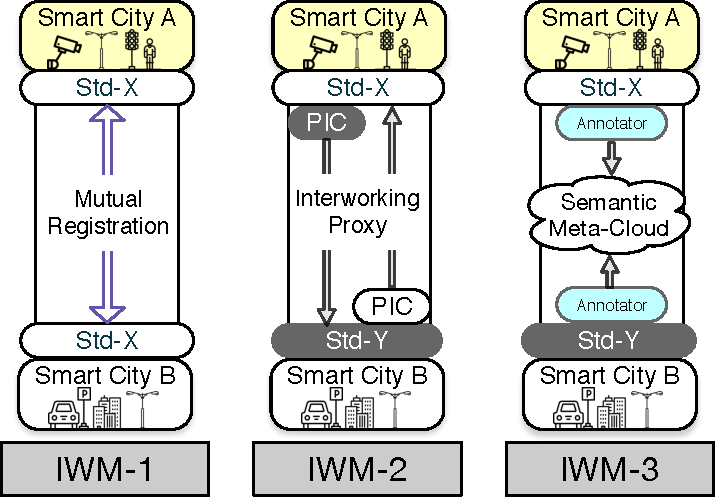
\includegraphics[width=\textwidth]{figures/fig_three_approaches_of_interworking.pdf}
    \caption{Three interworking models for smart city interoperability}
    \label{fig:three_interworkingmodel_for_smartcities}
\end{figure}

\begin{itemize}
  \item \textbf{\textit{Interworking Model-1:}} assumes that smart cities are using the same IoT standard. Standardizes interfaces are needed to have access to the other IoT platforms and exchange the data. Through those standardized interfaces, smart cities can operate their services but it has limitations in the case of citizens moving to other cities that are using different IoT standards.
  
  \item \textbf{\textit{Interworking Model-2:}} Unlikely IWM-1, this model is under consideration based on smart cities using different IoT standards. Data standard conversion component called Interworking Proxy Entity (IPE) is used to convert the data presentation of the source platform to the target platform. In this model, in addition to changing the data presentation, the meaning of the data is also translated.
  
  \item \textbf{\textit{Interworking Model-3:}} This model mainly focuses on creating a federation layer on top of the smart cities’ IoT platform. Any data generated by IoT services of cities can be stored into the meta-cloud database through standard conversion components based on well-defined APIs. In this article, the semantic concept is used for the federation layer.
\end{itemize}

The following subsections show how the three interworking models developed to achieve interoperability between cities are used. In addition, by using these models, authorities or service providers are able to interconnect their smart cities to other cities and they can be likely to expand the coverage of smart cities.

\subsubsection{The ways to realize the interoperability}
As mentioned earlier, it is relatively easy to solve the problem if smart cities that are intended to interoperate are using the same standard. This is because, in general, when developing a standard, resource type, structure and APIs are developed to support the communication among IoT platforms or devices using the same IoT standard. For example, oneM2M has a reference point called \texttt{Mcc} and a resource called \texttt{<remoteCSE>}. The \texttt{Mcc} reference point is the communication flows among other CSEs. These flows allow CSE to use the services being supported by other CSEs. \texttt{<remoteCSE>} resource represents a registree CSE which is registred to the Registrar CSE. \texttt{<remoteCSE>} resource have to be located directly under the \texttt{<CSEBase>}.  For exmaple, when CSE1 (Registree) registeres to CSE2 (Registrar), there will be two \texttt{<remoteCSE>} resource created. One for CSE1 (\texttt{<CSEBase1>}/\texttt{<remoteCSE2>}) and one in CSE2  (\texttt{<CSEBase2>}/\texttt{<remoteCSE1>}). As a result, since CSEs are registered both IoT platforms, users can access IoT services operated in CSE2 at \texttt{<CSEBase1>} by using the \texttt{<CSEBase1>/<remoteCSE2>}. To conclude, with the above functions, IoT platforms or devices using oneM2M can interoperate among them, and there is no need to develop additional components or develop resources.

\begin{figure}[H]			% Add figure one
	\centering
	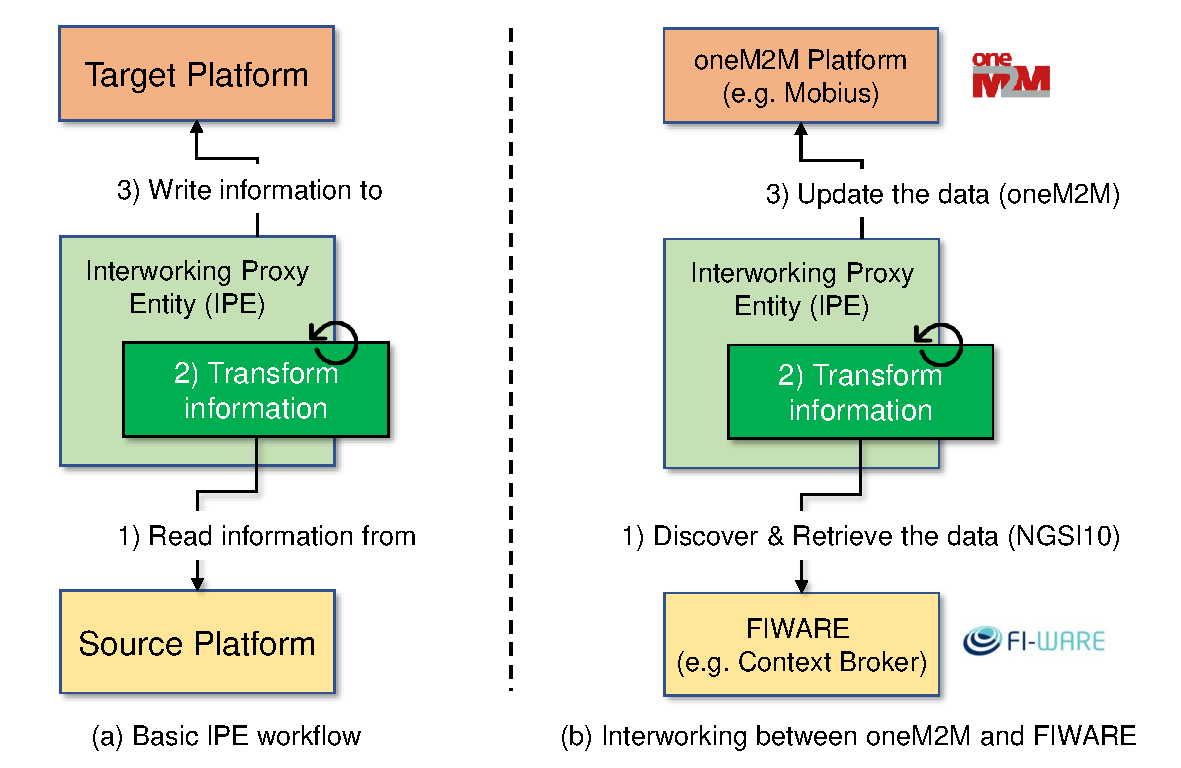
\includegraphics[width=\textwidth]{figures/fig_interworking_proxy.pdf}
    \caption{Interoperability procedures with FIWARE-oneM2M
example}
    \label{fig:interworking_proxy_entity}
\end{figure}

In contrast, additional work is required when connecting systems that use different standards. Research and development are underway for architecture to secure interoperability between various IoT platforms and devices. However, since it is inefficient to completely uniform the data and structure model for each standard, a standard conversion component based on Interworking Proxy Entity (IPE), which is a component that enables the dynamic connection between each standard, has been developed. Through these IPE components, it is expected that newly introduced platforms as well as existing IoT platforms can support interoperability. The IPE is a logical component developed to support interoperability for device-to-platform or platform-to-platform because communication standards and network interfaces are different depending on the manufacturers. However, as the demand for interworking increases, the number of interworking proxies also increases proportionally. This prevents the scalability of IoT standards and makes it difficult to efficiently manage resources, causing serious problems in providing IoT services. Therefore, to solve the above-mentioned problems, research on a method of managing various interworking proxy components through a common interface is also being conducted.
 
Figure.~\ref{fig:interworking_proxy_entity} shows the basic IPE structure and procedures, as well as the procedures of IPE interoperating with oneM2M and FIWARE platforms. The standard transformation component that operates in IPE reads information from the source platform and converts it to the data representation model of the target platform and stores it (Fig.~\ref{fig:interworking_proxy_entity} (a)). For example, the FIWARE-oneM2M (FO) IPE component utilizes the FIWARE platform as the source platform and the oneM2M standard platform as the target platform. When source and target platform information is provided, FO-IPE collects entity-based data stored in the standards-based FIWARE platform, converts it into the oneM2M standard-based data model, and stores it in the target platform (Fig.~\ref{fig:interworking_proxy_entity} (b)). This allows oneM2M applications to utilize data stored through the FIWARE platform. Examples of IPE components include Zwave-oneM2M (ZO), OCF-oneM2M (OO), LoRa-oneM2M (LO), GS1-oneM2M (GO) as well as the FO-IPE .

\subsection{Interworking Model-1 (IWM-1)}
In this subsection, IWM-1 is described as one of the ways to interconnect the smart cities. IWM-1 assumes that smart cities are using the same standard. In addition, oneM2M is selected as an example of the IoT standard. To conclude, by using oneM2M standard, this subsection shows how two smart cities can be connected.

\subsubsection{oneM2M for smart cities}
Besides the existing smart home and industry, the oneM2M is continuously developing and maintaining the standards in smart cities. oneM2M is currently contributing a smart city technology report (TR-0036), including domestic and overseas oneM2M smart city construction cases. Based on the existing cases, it will define various smart city models that can be configured using the oneM2M standard and derive the advantages of using standard technology.

% \begin{figure}[H]			% Add figure one
% 	\centering
% 	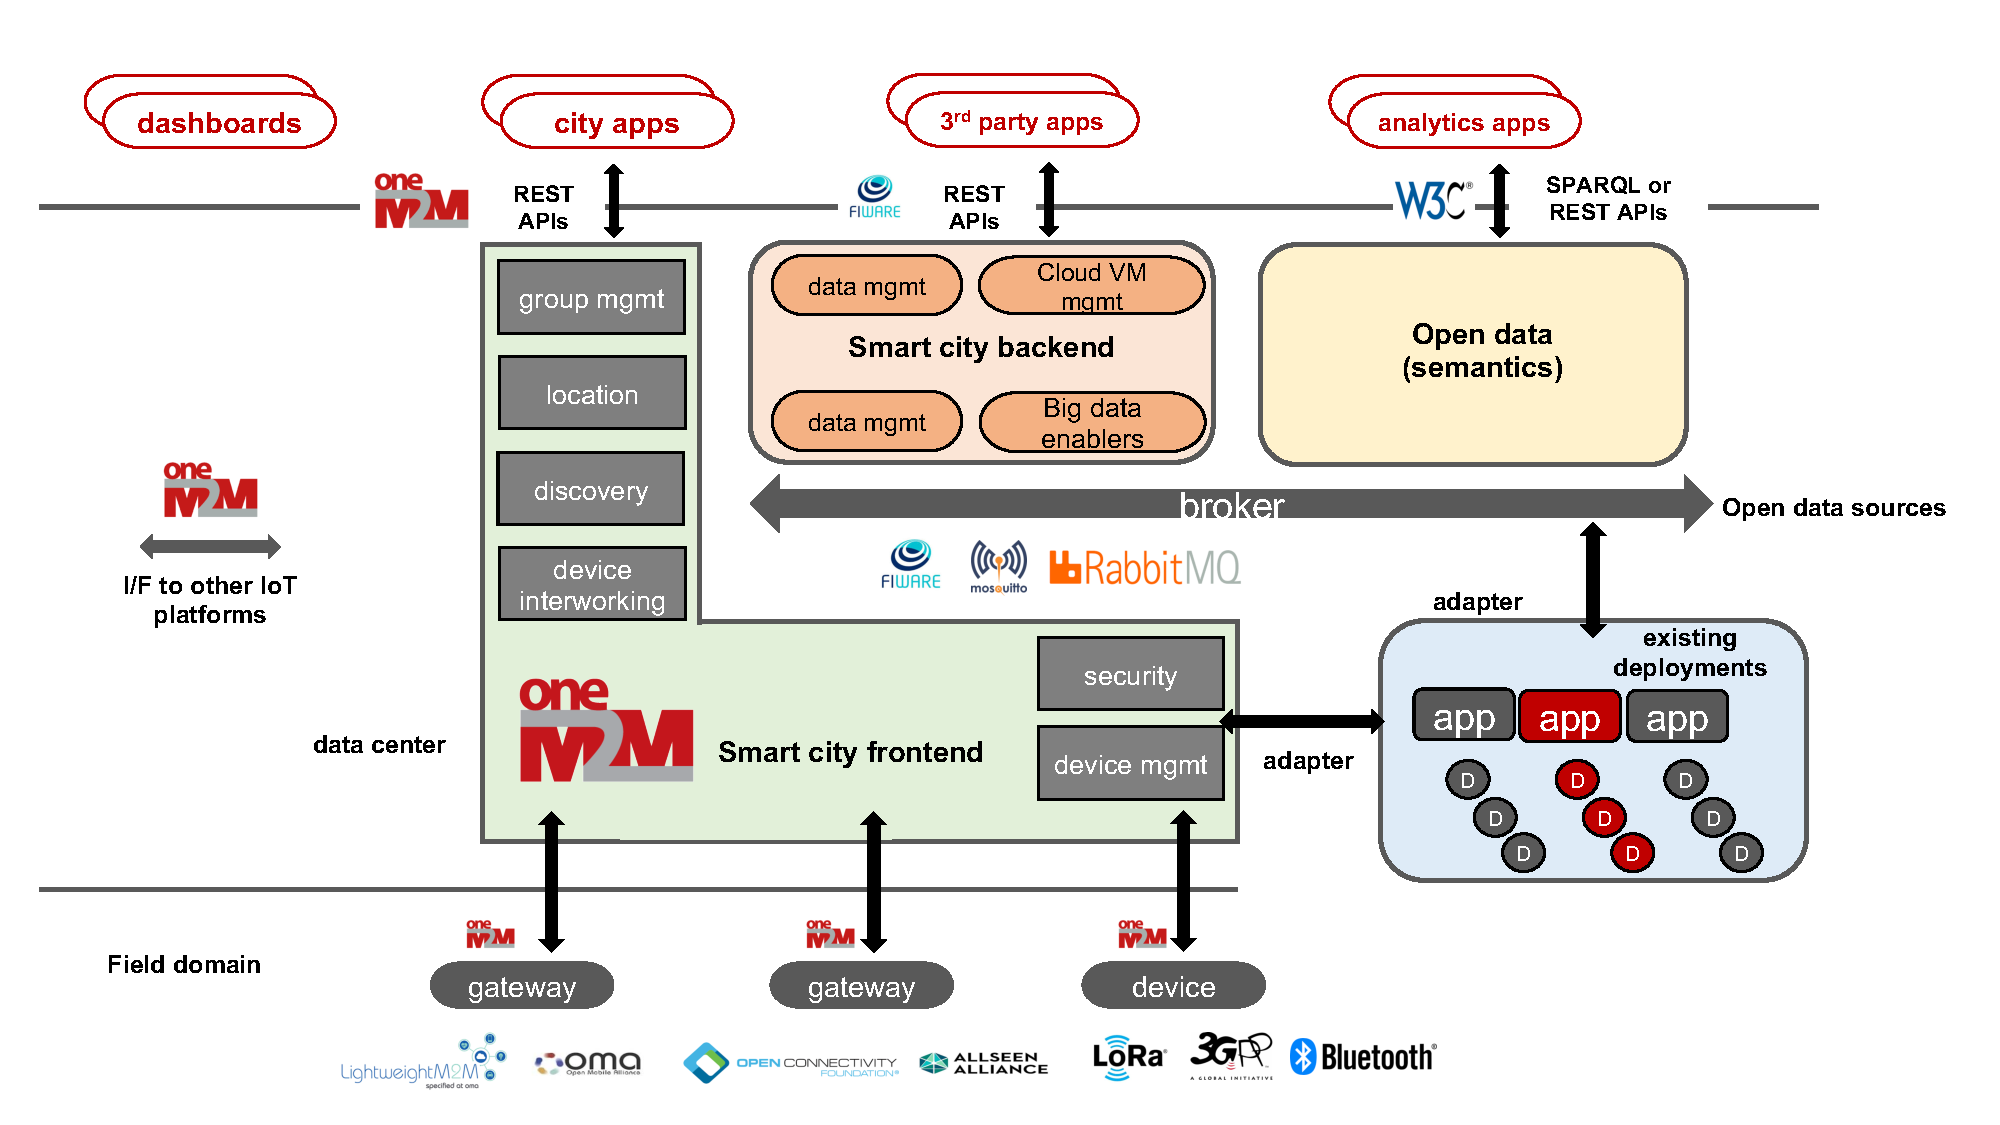
\includegraphics[width=\textwidth]{figures/fig_oneM2M_smartcity_blueprint.pdf}
%     \caption{oneM2M smart city blueprint}
%     \label{fig:onem2m_smartcity_blueprint}
% \end{figure}

Recently, smart cities are in the process of integrating IoT technology with existing urban infrastructure, and oneM2M can be regarded as a standard technology suitable for smart cities in this respect. Due to the nature of standard technologies, interoperability is basically guaranteed between devices, platforms, and applications that follow the standard. In addition, the Open Mobile Alliance (OMA), Lightweight M2M (LWM2M), Open Connectivity Foundation (OCF), AllJoyn, and oneM2M systems are interoperable by applying the interworking technical specifications developed in the oneM2M release 2. In addition, IoT devices equipped with network protocols such as ZigBee can also be linked to oneM2M, and by using semantic functions, large-scale smart city data collected from various services in the future can be analyzed and used between services as described in~\cite{onem2m_smart_cities_done_smarter}. To realize the interoperability of the cities, two types of interworking approaches as explained previously are being used.

% In addition, specifications for the inteorkwrking are as follows: TS-0014 LWM2M Interworking
% TS-0024 OCF Ineterworking
% TS-0026 3GPP Interworking
% TS-0035 OSGi-Interworking
% TS-0040 Modbus Interowrking
% TR-0042 WoT Interworking
% TR-0064 ZigBee Inteworking


\subsubsection{IWM-1 interworking procedures}
In this model, there is a assume that the IoT standard is defining the functions that allow smart cities to register and access the data with each other, and smart city interoperability can be realized if the IoT platform supports that IoT standards. The basic concept of IWM-1 is to connect smart cities using the same IoT standards. The IoT standard defines the functions that other smart cities can register or access data, and the smart city IoT platform can support each other by supporting the standard. When the IoT platform supports the above functions, the most important concept of IWM-1 is mutual registration. mutual registration is in charge of registering the resource of origin platform into the resource of the remote platform and vice versa. In addition, Additional procedures which is subscription/notification are needed to monitor the resource changes and apply the updated information to the existing resource. By using mutual registration, the information that is being used by users in smart city A can be delivered and stored in smart city B without changing any contents so that users who use a specific service in smart city A can get the same services in smart city B even though they move to smart city B.

\begin{figure}[H]		
	\centering
	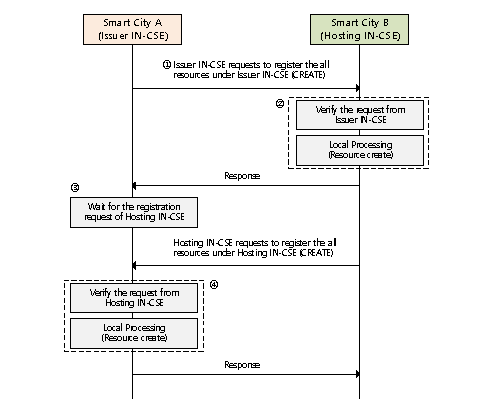
\includegraphics[width=\textwidth]{figures/fig_iwm1_mutual_registration_procedures.pdf}
    \caption{oneM2M mutual registration procedures}
    \label{fig:oneM2M_mutual_registration_procedures}
\end{figure}

The mutual registration procedure between IN-CSEs of the smart city is composed of the following four steps (see~Fig.~\ref{fig:oneM2M_mutual_registration_procedures}. In this figure, we assume that smart city A wants to interwork with smart city B and both cities are developed based on oneM2M standard. According to the oneM2M standard, all relevant data of cities are managed under the \texttt{<CSEroot>} resource as sub-resources. First, Issuer IN-CSE of the smart city A sends a request for registration to the hosting IN-CSE of smart city B by requesting the creation of a new \texttt{<CSEroot>} resource representing the issuer IN-CSE and all its sub-resources. The Issuer IN-CSE uses its identifier as the name of this new resource. In addition, It delivers the values that are needed to configure the new resource, for example, the URI of the issuer. As the second step, Hosting IN-CSE verifies that the delivered identifier of Issuer IN-CSE does not exist in its managing resources already. After checking the validity of the request, a new resource is created by using the requested identifier and given attribute values. In addition, all sub-resources of the Issuer resource are created to keep information of things in smart city A. If all these procedures are successful, a success response message is going to be returned to the Issuer. As a result, all the resources of the smart city A can be used in Hosting IN-CSE. After receiving a successful response from the Hosting IN-CSE, the Issuer is waiting for the mutual registration request from the Hosing IN-CSE as the third step. In this regard, Hosting IN-CSE sends a request for registering the own resources to Issuer IN-CSE as Issuer IN-CSE did. The Issuer checks the given identifier and creates all the required resources in case the request is properly validated. As the last step, the Issuer sends a success message to Hosting IN-CSE to complete the mutual registration properly.

In this way, as we mentioned before, users can use the same services even though the users move to other cities~\cite{kim2016standard, 2016funtionalarchonem2m, 2016applicationguidem2m}. Currently, this interworking model is being used by smart city projects such as Busan and Goyang for bridging the smart cities based on oneM2M.

\subsection{Interworking Model-2 (IWM-2)}
There exist many smart city IoT platforms which have different features, target domains, data models, and standards. For example, Busan and Santander cities are developed based on different standards, oneM2M and FIWARE, respectively. In this case, the data model and the way of managing IoT devices of a city are totally different. oneM2M city platforms consider devices as a resource, while FIWARE platforms are focusing on data and events from IoT devices. If a citizen from Busan visits Santander, any IoT services cannot be accessed by the citizen as there is no interoperability on the data model and IoT services. In this case, similar to other IoT solutions that used interworking proxy to support interworking between different IoT platforms or IoT devices, a proxy interworking function can be considered as a possible way to support interoperability between different smart cities.

\subsubsection{Interworking Proxy Entities (IPEs)}
By using the proxy-based model illustrated in Fig.~\ref{fig:resource_mapping_iot_platforms}, data, and services are interpreted and mapped to the ones of a target smart city. This interworking function is provided by a Proxy Interworking Component (PIC). PIC has a resource mapping rule between two city platforms using different IoT standards.
This resource mapping rule contains information about how a resource (i.e., representation of IoT data) is structured, configured and stored in the source and target city platforms. In this way, when there is a need for a citizen to have access to a resource in a remote city, the resource can be converted into understandable data.

\begin{figure}[H]			% Add figure one
	\centering
	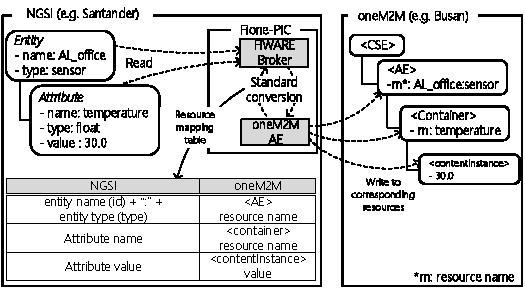
\includegraphics[width=\textwidth]{figures/fig_iwm_2_proxy_interworking.pdf}
    \caption{Resource mapping between IoT platforms}
    \label{fig:resource_mapping_iot_platforms}
\end{figure}

Let us consider a case where Bob, a citizen in Busan, wants to know a temperature value of Alice’s office in Santander. Busan is a smart city based on oneM2M, while Santander uses FIWARE. The oneM2M application that Bob is using does not support the NGSI interface used in Santander so that the application cannot discover a temperature device nor read the value of the sensor. To address this issue, FIWARE-to-oneM2M PIC (FIone-PIC) can be used and then Bob can get the NGSIbased data from Santander smart city. In other words, if users want to use IoT devices that use the NGSI context data model of FIWARE on the oneM2M platform, PIC is needed to convert the NGSI context data into the oneM2M resource structure.

\subsubsection{IWM-2 interworking procedures}
Fig.~\ref{fig:interworking_procedures_iwm2} describes how the FIWARE-to-oneM2M PIC converts the NGSI context data model into the oneM2M resource structure to use IoT devices without standard barriers. NGIS based IoT device registers to FIWARE ContextBroker that is the server based on NGSI standard (Step 1). PIC requests device information from the FIWARE ContextBroker based on the external input data received from the web portal. In this procedure, we assume that the web portal allows the users to select the devices registered in the FIWARE ConetxtBroker and FIWARE ContextBroker delivers device information to the PIC (Step 2, 3). PIC converts the standard from the FIWARE NGSI standard to oneM2M in order to register FIWARE device information into the oneM2M server (Step 4). PIC performs the subscription operation for handling the device data update case (Step 5). As soon as FIWARE device is updated, PIC update existing oneM2M information by using notification and transformation mechanism is already described before (Steps 6, 7, 8).

\begin{figure}[H]			% Add figure one
	\centering
	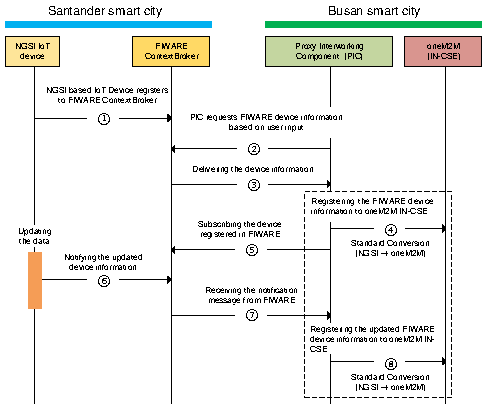
\includegraphics[width=\textwidth]{figures/fig_proxy_interworking_procedures.pdf}
    \caption{Inetworking procedures between two smart cities}
    \label{fig:interworking_procedures_iwm2}
\end{figure}

As a practical example using this model, there is a project called Wise-IoT (http://wise-iot.eu/en/about/), and it leads the project under the theme of smart city interworking through semantics technology. In this project, IWM-2 is adopted to support interworking between oneM2M and non-oneM2M standard devices based on NGSI, Open Connectivity Foundation (OCF), Lora, and Z-wave.

\subsection{Interworking Model-3 (IWM-3)}
Unlike the previous two IWMs, IWM-3 is based on the centralized cloud system. More specifically, the semantic-based central cloud is used to federate the other smart cities by using semantic technology. The data generated by smart cities are translated according to the semantic rule and this is delivered to the semantic-meta cloud. In this subsection, first, the basic concept of semantic is illustrated and subsequently, IWM-3 describes with the architecture.

\subsubsection {Semantics}
The Semantic web was first proposed by Tim Berners Lee in 1998~\cite{berners2001semantic}, and it establishes relationships among numerous information and resources available on the Internet. As a result, machines or computers understand each other without human intervention. The purpose of the Semantic web is to develop standards and technologies to help computers easily understand information on the Web, supporting semantic search, data integration, navigation, and automation of tasks. In order to support these functions in the Semantic web, it is necessary to insert a concept for knowledge expression in a web document, establish relationships between knowledge, and include inference rules to enable intelligent information processing of computers. Through this, it is possible to accurately convey the information desired by the users~\cite{ontology_web_frotoma}. As described in Fig.~\ref{fig:semantic_comparison}, the HTML link basically links the document node to a link called \texttt{href} tag, and links two resources, and is a simple link that does not express its own meaning. On the other hand, by providing type information to each node and link, a more meaningful network can be constructed~\cite{2008_semantic_books}.

\begin{figure}[H]			
	\centering
	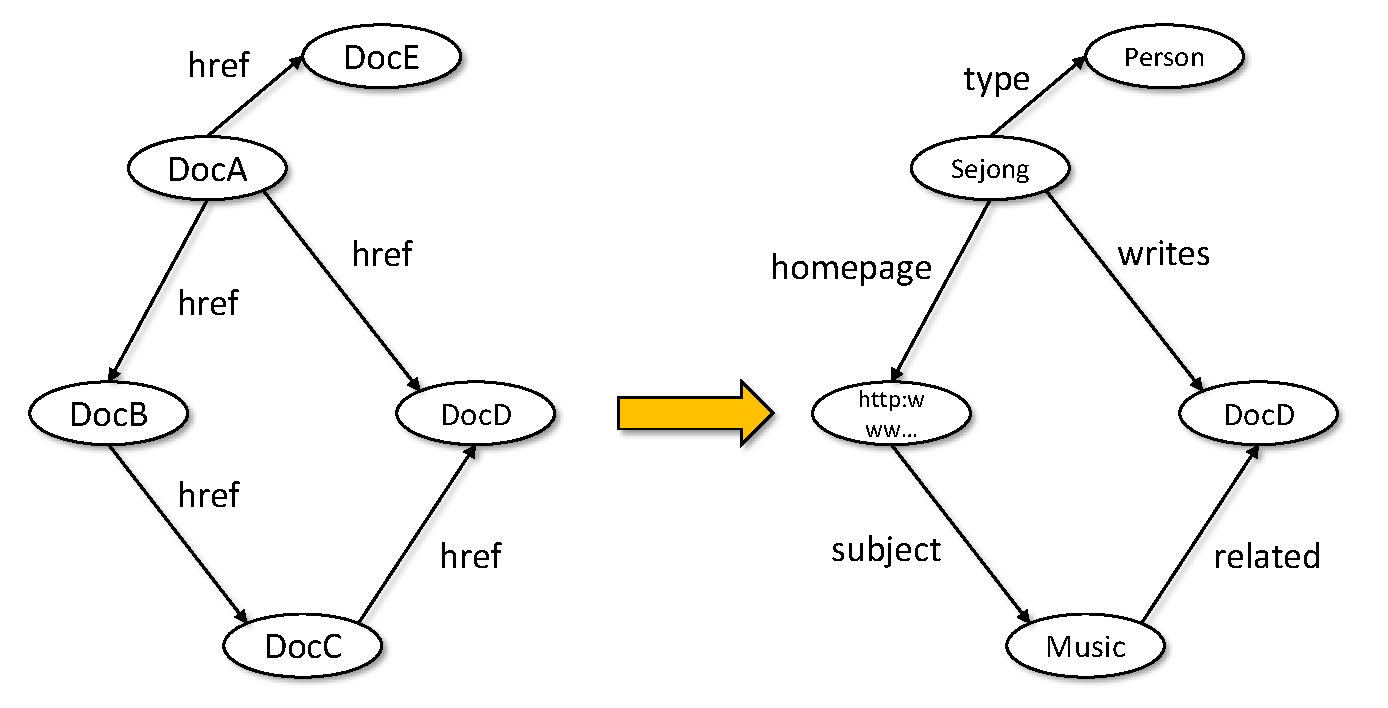
\includegraphics[width=\textwidth]{figures/fig_semantic_comparison.pdf}
    \caption{Comparison between HTML and semantics}
    \label{fig:semantic_comparison}
\end{figure}

The core technology that enables the implementation of the semantic web is an ontology that formally describes the concepts in the domain and the relationships. It uses languages such as Resource Description Framework (RDF) and Web Ontology Language (OWL). By implementing ontology, computers can process data based on knowledge. Based on the application of semantic technology through the development of an ontology of specific domains, simply beyond the use of raw data generated by sensors or devices, many studies have been conducted to support IoT services by combining the current IoT technology and semantic technology.

Thanks to the advantages of this technology, research is being conducted to apply it to the IoT industry. For instance, in the oneM2M case~\cite{tr0007}, the current approach taken by oneM2M treats data as black boxes. This means that the content is opaque and applications need to know in advance how the data interpret. Therefore, semantics are essential if the M2M system is expected to interact with real entities (“things”) because the main role of semantics is to provide a description of the relationship between things/data/information. 

\begin{figure}[H]
	\centering
	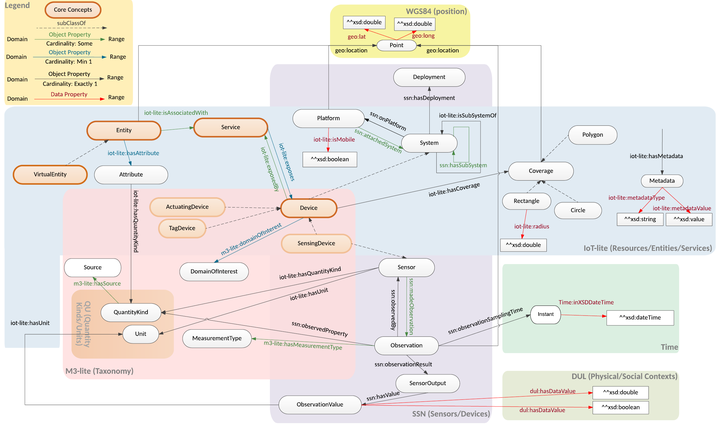
\includegraphics[width=\textwidth]{figures/fig_fiesta-ontology.png}
    \caption{FIESTA-IoT common ontology}
    \label{fig:fiesta-common-ontology}
\end{figure}

With such advantages, the FIESTA-IoT (http://fiesta-iot.eu/) project is commenced to provide semantic interoperability between different smart city IoT testbeds and expose the services as an Experiment-as-a-Service (EaaS) model, which defines a single entry point to all FIESTA-IoT services. However, existing ontologies are not well connected and are domain-specific. That is, the ontology for the IoT service is an ontology according to specific domains, and the existing developed ontology may not be suitable for other services, so the ontology needs to be additionally extended. However, extending the ontology according to each requirement increases the complexity and is not suitable. In this context, to achieve semantic interoperability, the FIESTA-IoT project defined a common ontology called FIESTA Ontology. For constructing the FIESTA common ontology, it leverages various concepts of Semantic Sensor Network (SSN) ontology, IoT-lite ontology, Machine-to-Machine Measurement (M3) Lite (M3-lite) Ontology, and by using these concepts, it covers most of the concepts for achieving the goal of the semantic interoperability and the federation~\cite {agarwal2016unified}.

To translate from testbeds' intrinsic formats to the one that is understood and interpreted by the FIESTA ontology, semantic annotation is needed. First, let us check what annotation is. Annotation means adding additional information to a sentence or document. It is often considered as ‘comment’, and comments written as a description of source code in a programming language are a kind of annotation. In computer technology, annotation means mapping the analysis result of a specific text to the text. The purpose of annotations is to provide additional information about a document, sentence, text, or specific concept, and to make the information available in a variety of places. Based on this concept, semantic annotation is used to annotate the metadata to the web resources. Metadata is summarized as ``Data about the data". In the semantic web, information about web resources, etc. described in a form that a computer can read and understand is called metadata. Meanwhile, the procedure of describing metadata in a form that can be processed by a computer using a metadata expression language such as RDF, OWL, etc., and giving metadata to web content is called a semantic annotation~\cite{kiryakov2004semantic, euzenat2002eight}.

\begin{figure}[H]			% Add figure one
	\centering
	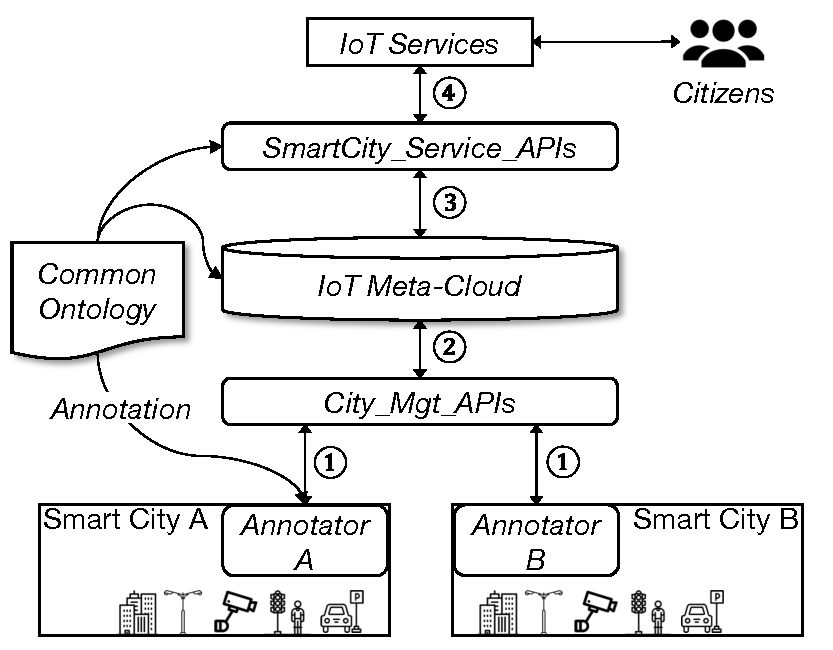
\includegraphics[width=\textwidth]{figures/fig_iwm3_semantic_interworking_interop.pdf}
    \caption{Semantic interoperability architecture}
    \label{fig:semantic_interoperability_architecture_iwm3}
\end{figure}

\subsubsection{IWM-3 interworking procedures}
Semantic interoperability enables different agents, services, and applications to exchange information, data, and knowledge that arrive at equivalent meanings~\cite{barnaghi2012semantics, strassner2016semantic}. IWM-3 is an IWM based on semantic interoperability assets, and by using this model, cities can interwork and exchange information, as this information is understandable. In addition, IWM-3 defines a centralized server platform that federates various smart cities using semantic interworking and provides a common set of semantic APIs. In addition, underlined smart cities could be developed either based on the same standards or based on different IoT platforms using different IoT standards. Figure.~\ref{fig:semantic_interoperability_architecture_iwm3} shows the high-level architecture of IWM-3 to make smart cities semantically interoperable. The IWM-3 comprises the four main components: 1) Unified Ontology to semantically annotate the data, 2) Meta-Cloud to store semantically annotated data pushed by the registered resources of underlined smart cities, 3) CITY-MGT-APIs for smart cities to register and manage themselves and their resources and to push observations in Meta-Cloud, and 4) SmartCity-Service-APIs which enable the end users and developers to obtain data from any smart cities registered to this meta-cloud~\cite{gyrard2015unified}.

\begin{table}[ht]
\setlength{\tabcolsep}{3pt}

\begin{center}
\begin{tabular}{|p{3.7cm}|p{8cm}|}
\hline 
\centering Services & \hspace{3.3cm}Description\\
\hline

\centering  getLastObservations & This service provides the latest values of a specific Sensor list in an FIESTA-IoT \\
\hline

\centering  getObservations & This service provides the values of a specific Sensor list for a specific time-period in an FIESTA-IoT \\
\hline

\centering  pushLastObservations & This service initiates a stream at the Testbed side which pushes
continuously the latest values of a specific Sensor \\
\hline

\centering  pushSingleObservation & This service pushes continuously the latest value of a specific Sensor \\
\hline

\centering  stopPushOfObservations & This service stops the push of observations initiated by the
“pushLastObservations” and “pushSingleObservation” \\
\hline

\end{tabular}
\end{center}
\caption{Testbed Provider Services (TPS)}
\label{tab:fiesta_iot_tps_api}
\end{table}

To fill the gap of understanding between different cities and their data formats, IWM-3 defines Meta-Cloud on top of all smart cities to store and manage standardized semantic information. The IoT data on each smart city platform is converted into semantic data using a standardized ontology. The ontology can encode the meanings of data in a form that does not change. Underlined smart cities consume CITYMGT-APIs to register their resources in the Meta-Cloud and push data to Meta-Cloud after converting to the semantic data using the common ontology (Steps 1 and 2). For this data conversion, each underlined smart city has to develop and deploy its own semantic annotator by means of the transformation of the information it stores locally to data described by using the common semantic ontology. Then, IoT services use the SmartCity-Service-APIs to allow users to access data distributed around the underlined smart cities (Steps 3 and 4). In the FIESTA-IoT project, there is a set of RESTful web services called Testbed Provider Interface (TSI) for integrating the testbeds into the FIESTA-IoT platform. For example, as core services of the TSI, Testbed Provider services (TPS) are defined to provide the ``pluggability" of the testbed to the FIESTA-IoT platform, and a list of services are can be considered as CITY-MGT-APIs. TPS is listed in Table~\ref{tab:fiesta_iot_tps_api}~\cite{fiesta2017architecture}. 

\subsection{Interworking model evaluation}
% Please add the following required packages to your document preamble:
% \usepackage{booktabs}
\def\doitems{\def\item{\par
   \noindent\hbox to 2.3em{\hss$\bullet$\hss}\hangindent=2.3em }}

\begin{table*}[ht]
  \renewcommand{\arraystretch}{1.5}
  \scriptsize

  \begin{tabular}{p{0.9cm}p{3.3cm}p{3.4cm}p{3.4cm}}
    \hline
      & \centering IWM-1 & \centering IWM-2 & \hspace{1.5cm} IWM-3 \\
    \hline
    
    \centering Scalability & 
    \doitems   
        \item Pros: This is highly scalable if a single standard is mandated.
        \item Cons: It is difficult to mandate that all cities follow the same standard. & 
    \doitems   
        \item Pros: Interconnected smart cities can easily be extended using PIC.
        \item Cons: It is not easy to develop PIC for all standards. &
    \doitems   
        \item Pros: The use of semantics ensures scalability. 
        \item Cons: It is difficult to develop annotators for all standards. \\
        
    \hline
    \centering Complexity & 
    \doitems   
        \item Pros: A standard body only needs to define standardized mutual registration procedures. & 
    \doitems   
        \item Cons: As interworking cities grow, the complexity grows steeply. & 
    \doitems   
        \item Pros: Each city only needs to provide an annotator for the common ontology.
        \item Cons: The common ontology can become complicated. \\
        
    \hline
    \centering Data redundancy & 
    \doitems   
        \item Cons: All data on a platform should be replicated on a remote platform. & 
    \doitems   
        \item Pros: A platform only needs to have data that it interworks with. & 
    \doitems   
        \item Pros: The meta-cloud only needs to store the semantic description. 
        \item Cons: All data should be annotated and stored in the meta-cloud. \\
        
    \hline
    \centering Development effort \& cost & 
    \doitems   
        \item Platform developers take on a small burden. Application developers only need to use the standardized APIs. & 
    \doitems   
        \item Platform developers have to develop PICs while App developers just need to know their city APIs. & 
    \doitems   
        \item Each city platform owner has to develop annotators, while App developers only need to use given APIs. \\
        
    \hline
    \centering {Privacy \& security} & 
    \doitems   
        \item Pros: High probability that two cities are using the
                                       same security mechanism. & 
    \doitems   
        \item Cons: May need security mechanisms for secure interworking. & 
    \doitems   
        \item Cons: Additional common security mechanisms need to be defined. \\
    \hline
  \end{tabular}
  \caption{Summary of IWM analysis}
    \label{tab:iwm_model_evaluation}
\end{table*}
This subsection compares and analyzes the three IWMs against the five criteria, which are selected to see an impact on the stakeholders of smart city development such as platform companies and city owners.

\textbf{Scalability:} Depending on the number of smart cities to be interconnected, each IWM shows different scalability. IWM-1 is highly scalable, as this model mandates a single standard for all smart cities. This model can extend to as many interconnected smart cities as necessary if the city governments all agree to use the same standards. However, this is not realistic, as city governments decide their standards based on many different factors, such as culture and international relationships. IWM-2 and 3 can also provide scalability under the assumption that PIC and Annotator are easily developed and deployed. However, as the number of interworking cities grows, it becomes more difficult to support PICs and Annotators for all cities.

\textbf{Complexity:} In the case of IWM-1, standard development organizations~(SDOs) only need to define mutual registration procedures. Then, all the smart cities can be interconnected by implementing the procedures, which is easy. IWM-3 shows average complexity, as each smart city only needs to develop one annotator to convert its data to semantically annotated data with the common ontology. To interwork with N cities, the same number of annotators is required. On the other hand, IWM-2 shows the highest complexity. In this IWM, each smart city has to support PIC for all the interworking cities. This means we need (N-1)*N PICs to interconnect N cities.   

\textbf{Data redundancy:} The amount of data a smart city has to manage is very important in terms of city performance. It is not possible to support the city interworking without data redundancy. All IWMs cause data redundancy. IWM-1 shows the worst data redundancy rate among the three models as it forces both interworking cities to store their remote data on their platform. IWM-2 requires the same data redundancy as IWM-1. However, with a small enhancement feature (i.e., introducing a dynamic morphing mediation interworking proxy that is able to load only necessary interworking functions), the rate of data duplication can be decreased dramatically. Compared with IWM-1 and 2, the semantic IWM has a lower data redundancy rate, as IWM-3 only needs to store a semantic description of the data, not the data itself.

\textbf{Development effort and cost:} Typically, platform developers implement an IT infrastructure to operate smart cities, while application developers work on smart city services using given APIs from smart cities. In the case of IWM-1, a small amount of effort is required from both developers for interworking, as all platforms are standardized. On the other hand, IWM-2 and 3 force platform developers to exert significant effort on developing PICs and annotators. The application developers, in this case, just need to know about their own city APIs. Currently, many smart cities are being led by the government with public funding, which may come from the government, federal, or state, so that the development and deployment of the PIC and annotator are usually conducted as open-source projects which are available to the general public for use. In the future, after finishing the government funding phase, any smart city that wants to be connected (IWM-3) to the meta-cloud and interwork (IWM-2) with other smart cities should develop and operate such software with their own funding. However, through using various open-source interworking modules developed in government funded smart city projects, the cost of developing such software can be reduced significantly.

\textbf{Privacy \& security:} For consistently operating the smart cities, privacy and security are critical challenges in supporting data confidentiality and authentication, access control, privacy, and trust when citizens and entities move between cities. In particular, when a citizen moves to other cities that have different security and privacy regulations, important private data can be easily leaked. Even the same IoT standard is used in IWM-1, if different privacy regulations are used in the inter-connected cities, a framework managing privacy issues within a heterogeneous smart city environment is needed. IWM-2 and IWM-3 generally need a mechanism supporting secure interworking. However, such a mechanism is not always required as there exist cases that ban on data transfer across cities or nations by policymakers because of privacy and cybersecurity, or economic mercantilism. Therefore regardless of which IWM is selected, proper mechanisms for guaranteeing security and privacy across smart cities have to be considered carefully. To conclude, Table~\ref{tab:iwm_model_evaluation} shows a summary of our IWM analysis. No single IWM is better than the others are. All the models have their own pros and cons. City owners or designers should consider their environment (e.g., budget, relationship with other cities, plan for interworking, regulations) in selecting their IWM.

\subsection{Summary}
In this article, three interworking models that are needed to solve the IoT standard interoperability issue are proposed with smart city scenario, and also evaluated the three interworking models. By using one of these models, not only developers can easily support the variety of IoT standards but also existing IoT platforms can also support other IoT standards without any changes in the existing system.
\clearpage